\noindent

\includegraphics[height=1.25cm]{images/pictograms/replication}
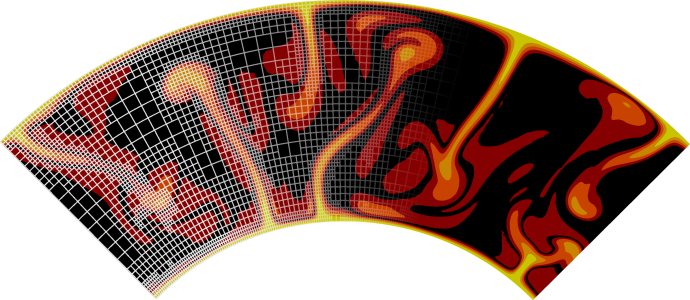
\includegraphics[height=1.25cm]{images/pictograms/aspect_logo}

\includegraphics[height=1.25cm]{images/pictograms/benchmark}

\includegraphics[height=1.25cm]{images/pictograms/pic}

%%%%%%%%%%%%%%%%%%%%%%%%%%%%%%%%%%%%%%%%%%%%%%%%%%%%%%%%%%%%%%%%%%%%%%%%%%%%%%%%%%%%%%%%%%%%%%%%%%%

\begin{flushright} {\tiny {\color{gray} python\_codes/fieldstone\_122/text.tex}} \end{flushright}

%\lstinputlisting[language=bash,basicstyle=\small]{python_codes/template_keywords.key}

\par\noindent\rule{\textwidth}{0.4pt}

\begin{center}
\inpython
{\small Code: \url{https://github.com/cedrict/fieldstone/tree/master/python_codes/fieldstone_122}}
\end{center}

\par\noindent\rule{\textwidth}{0.4pt}

{\sl This stone was developed in collaboration with Donald Duck}. \index{contributors}{D. Duck}

\par\noindent\rule{\textwidth}{0.4pt}

%%%%%%%%%%%%%%%%%%%%%%%%%%%%%%%%%%%%%%%%%%%%%%%%%%%%%%%%%%%%%%%%%%%%%%%%%%%%%%%%%%%%%%%%%%%%%%%%%%%

This \stone is a replication of the benchmarks found in the supplementary material 
of \textcite{galh18} (2018). 

\begin{displayquote}
We tested the accuracy of the implemented advection
schemes with two example models that separately show the
convergence of the integration error in spatially and tem-
porally variable flow. Both models use an analytically pre-
scribed velocity function that is evaluated and transferred
to the finite-element solution vector. By this procedure we
ensure that the particle algorithm behaves as in a normal
coupled computation, but retain full control over the veloc-
ity field that allows us to choose benchmarks with analytical
solutions, and are independent of the accuracy of the finite
element solver
\end{displayquote}

\begin{center}
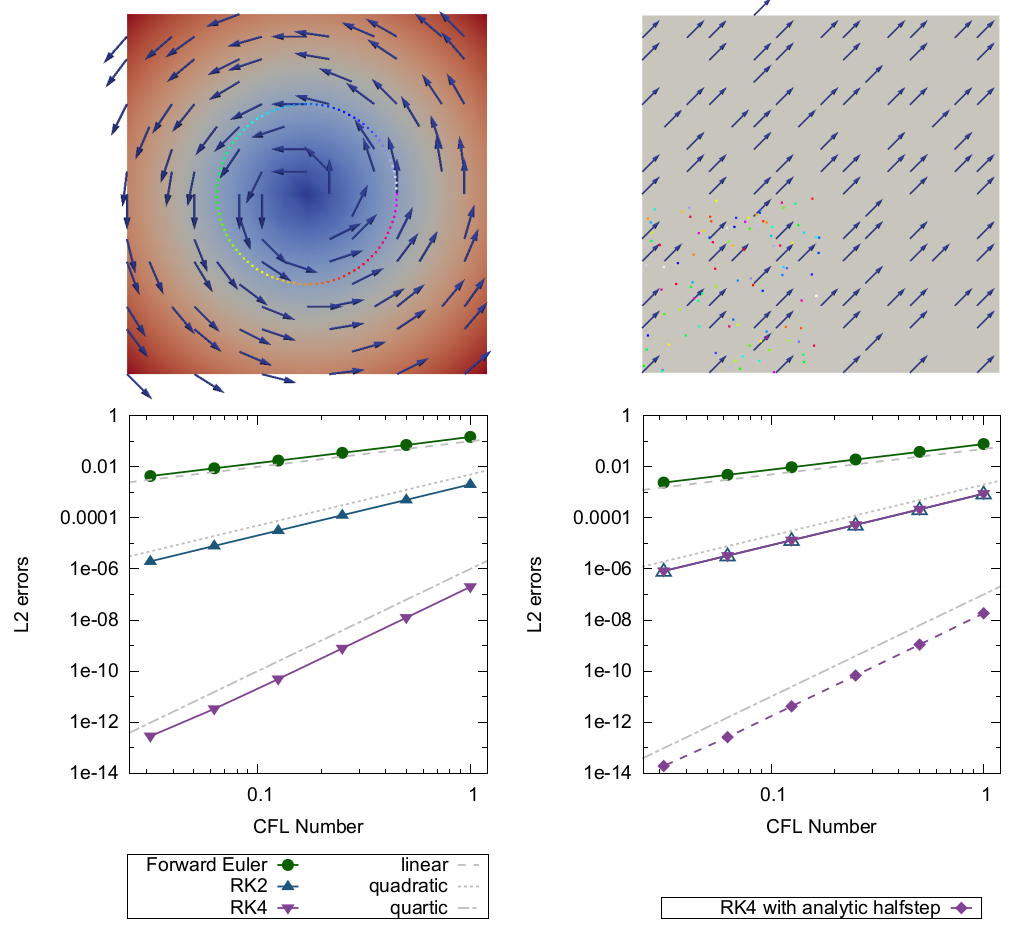
\includegraphics[width=11cm]{python_codes/fieldstone_122/images/galh18.png}\\
{\captionfont Taken from the supplementary material of \textcite{galh18} (2018).}
\end{center}

%%%%%%%%%%%%%%%%%%%%%%
\section*{Benchmark 1}

This benchmark is described as follows:
\begin{displayquote}
The first benchmark model consists of a circular flow
around the center of a two-dimensional box. The model
end time and velocity of the flow is chosen to match one
turn-around time around the center. The model contains
100 particles that are distributed in a ring with a constant
radius around the model center. The error is measured as
distance between final and initial position that should approach 
zero in an analytical solution. To ensure that the
error is independent of the particle’s starting position we
plot the maximal error of all particles.
\end{displayquote}

\begin{center}
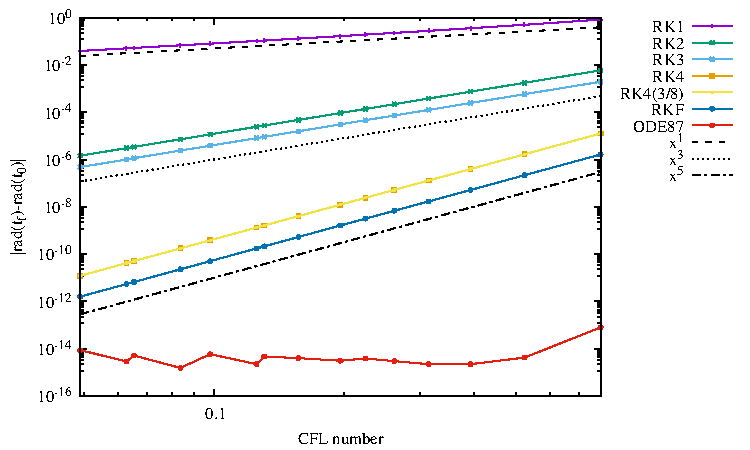
\includegraphics[width=8cm]{python_codes/fieldstone_122/results/exp1/errors.pdf}
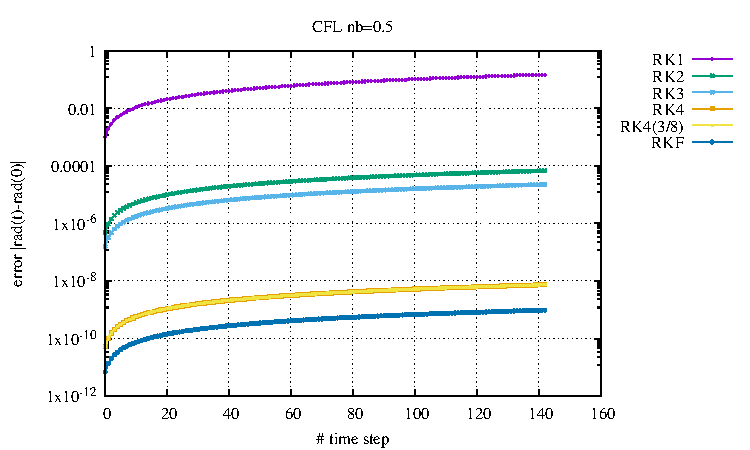
\includegraphics[width=8cm]{python_codes/fieldstone_122/results/exp1/rad.pdf}\\
{\captionfont Left: radius error as a function of the CFL number and for various RK methods;
Right: radius error as a function of time for a given CFL number of 0.5.}
\end{center}

I do not exactly measure the same thing as in the paper. 
Ifind that even order RK over perform. Also, not much difference between RK4 and RK4-3/8.

%%%%%%%%%%%%%%%%%%%%%%
\section*{Benchmark 2}

This benchmark is described as follows:
\begin{displayquote}
The second benchmark model measures the convergence
in time-variable flow, which is simulated by a model domain 
with spatially constant but over time exponentially-
increasing velocity. All particles are generated at random
positions in the lower-left quadrant of the model domain
and are advected in a flow of the form
\[
u(t)=1 + e^t \qquad 
v(t)=1 + e^t 
\].
The model end time
of 1 then leads to an expected final
position $\vec{x}(1) = \vec{x}(0) + \int_0^1 \vec\upnu(t) \; dt$
 with a distance between the initial and end position of $d = ||\vec{x}_1-\vec{x}_0 ||_2 = 2e$.
\end{displayquote}








